\documentclass[aspectratio=169]{beamer}


\usenavigationsymbolstemplate{}

\usetheme{unibt}
\usepackage{xcolor}
\usepackage[ansinew]{inputenc}
\usepackage{times}
\usepackage[T1]{fontenc}
\usepackage[authoryear]{natbib}
\usepackage{transparent}
\usepackage[titletoc]{appendix}
\usepackage[left]{eurosym}
\usepackage{booktabs}
\usepackage{animate}
\usepackage{graphicx}
\usepackage{epstopdf}
\usepackage{hyperref}
\usepackage{tikz}
\usetikzlibrary{decorations.pathreplacing, shape, fit, positioning}
\usepackage{pgfplots}
\pgfplotsset{compat=1.18}
\usepackage{svg}
\usepackage[ruled,vlined]{algorithm2e}
\usepackage{algpseudocode}


\usepackage[absolute, overlay]{textpos} % gives textblock environment
\usepackage{xurl} % break urls


\newcommand{\rbg}[1]{\raisebox{2.25ex}[-2.25ex]{#1}}
\newcommand{\rbv}[1]{\raisebox{1.25ex}[-1.25ex]{#1}}

\newcounter{saveeqn}
\newcommand{\appeqn}{\setcounter{saveeqn}{\value{equation}\stepcounter{saveeqn}}%
	\setcounter{equation}{0}%
	\renewcommand{\theequation}{%
		\mbox{A\arabic{equation}}}}
\newcommand{\reseteqn}{\setcounter{equation}{\value{saveeqn}}%
	\renewcommand{\theequation}{\arabic{equation}}}

\newcommand{\appppage}{
	\setcounter{page}{1}%
	\renewcommand{\thepage}{%
		\mbox{A\arabic{page}}}}

\newcommand{\appsection}{
	\setcounter{section}{1}%
	\renewcommand{\thesection}{%
		\mbox{A\arabic{section}}}}

\newcounter{tableapp}
\newcommand{\apptable}{\setcounter{tableapp}{\value{table}\stepcounter{tableapp}}%
	\setcounter{table}{0}%
	\renewcommand{\thetable}{%
		\mbox{A\arabic{table}}}
	\renewcommand{\theHtable}{%
		\mbox{A\arabic{table}}}}

\newcommand{\resettable}{\setcounter{table}{\value{tableapp}}%
	\renewcommand{\thetable}{\arabic{table}}}

\definecolor{titlecolor}{RGB}{3,138,94} 


\usefoottemplate{\vbox{%
		\tinycolouredline{structure!0!hell}%
		{\color{white}\begin{parbox}{0.5cm}{
\includegraphics[height=0.35cm]{figures/logo2.eps}}\end{parbox}\hspace{0.1cm}\begin{parbox}{4.4cm}{\textbf{Simon\  Bl\"othner}}\end{parbox}\hspace{2.5cm}\begin{parbox}{2cm}{ \insertframenumber\,/\,\inserttotalframenumber}\end{parbox}\hfill\begin{parbox}{2.2cm}{\textbf{EARIE 2025}}\end{parbox}}}}


\useheadtemplate{\vbox{%
		\tinycolouredline{structure!0!hell}%
		{\color{white}\begin{parbox}{20cm}{\insertsection}\end{parbox}}}}



\title{Conglomerate Mergers: \newline Effects on
Growth and Competition}


\author{Simon Bl\"othner \\
  \small University of Bayreuth
}
%\institute{\inst{1}University of Bayreuth  \and \inst{2}Defiria \and \inst{3}Charles River Associates}
\date{\today}

\begin{document}
\maketitle

\begin{frame}{Motivation}
  \begin{columns}[T]
    \begin{column}{0.4\textwidth}
      \begin{tikzpicture}
        % Adjust the coordinates to position logos as needed
        \node at (0,0) {\includesvg[width=2cm]{figures/logos/Adani_logo_2012.svg}};
        \node at (1,1) {\includesvg[width=2cm]{figures/logos/Hitachi_logo.svg}};
        \node at (-1,2) {\includesvg[width=2cm]{figures/logos/Procter_&_Gamble_logo.svg}};
        \node at (-1,-1) {\includesvg[width=2cm]{figures/logos/Samsung_wordmark.svg}};
        \node at (2,-1) {\includesvg[width=2cm]{figures/logos/Lockheed_Martin_logo.svg}};
        \node at (2,-2) {\includesvg[width=2cm]{figures/logos/LVMH_wordmark.svg}};
        \node at (1,3) {\includesvg[width=2cm]{figures/logos/JNJ_Logo_New.svg}};
        \node at (-1,-3.3) {\includesvg[width=2cm]{figures/logos/DuPont_logo.svg}};
        \node at (2.2,2) {\includesvg[width=2cm]{figures/logos/Siemens_AG_logo.svg}};
        \node at (0,-2) {\includesvg[width=2cm]{figures/logos/KT_Logo.svg}};
        % Add more nodes for additional logos
      \end{tikzpicture}
      
    \end{column}
    \begin{column}{0.6\textwidth}
      \begin{itemize}
        \setlength\itemsep{0.8em}
        \item A conglomerate is a combination of business units operating in entirely different industries
        \item Usually they span multiple countries (multinational)
        \item There are more than \textit{1,000} conglomerates worldwide
        \item Highly dynamic process of merging, acquiring and splitting
        \item Many of the brands you use daily probably belong to a conglomerate
      \end{itemize}
    \end{column}
    
  \end{columns}
       
\end{frame}

\begin{frame}{Key Questions}
  
  \begin{enumerate}
    \setlength\itemsep{0.8em}
    \item Why would firms in \textit{unrelated} markets merge? 
    \item How could antitrust authorities evaluate conglomerative mergers?
    \item How do management costs affect conglomerate structure?
  \end{enumerate}

\end{frame}

\begin{frame}{Seeking Your Input}
    \begin{block}{Publication Strategy Discussion}
      I would greatly appreciate your thoughts on:
      \begin{itemize}
        \setlength\itemsep{0.8em}
        \item Where this work fits within the existing literature
        \item Which journals or outlets might be most suitable
        \item What modifications would strengthen the contribution for
  publication
      \end{itemize}
    \end{block}

    \vspace{0.5cm}
    \centering
    \textit{Your expertise and suggestions would be invaluable!}
\end{frame}

%  \begin{frame}{The Power of Resource Pooling}
%   \begin{center}
%     \only<1>{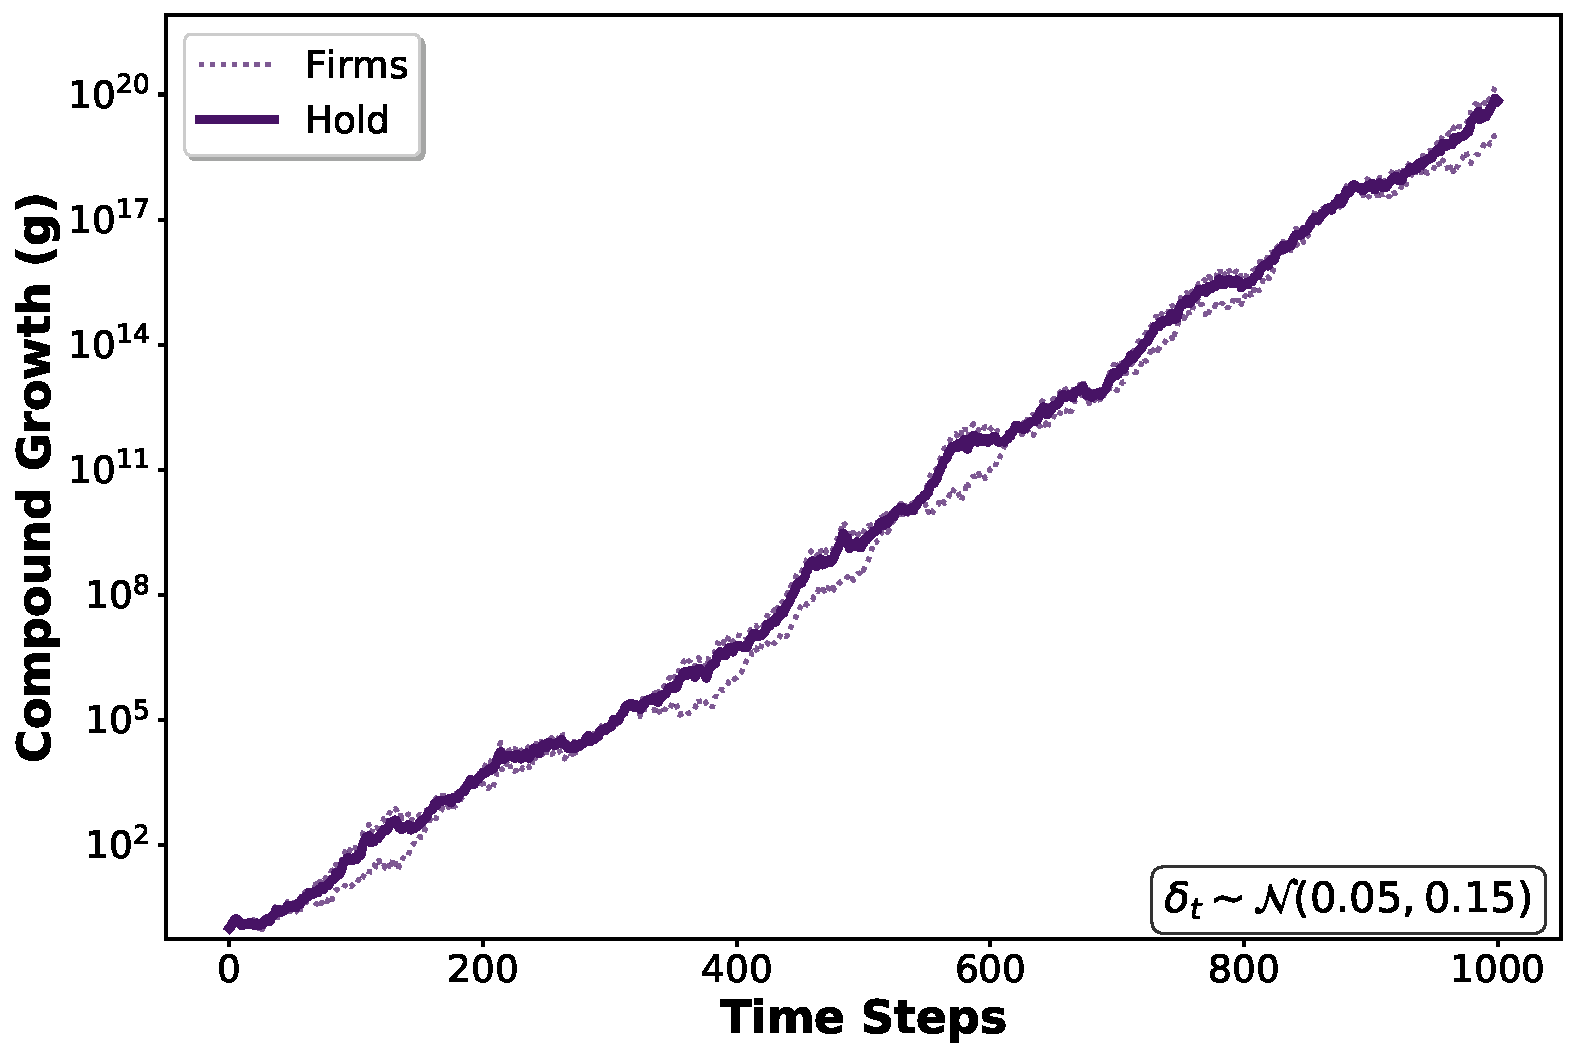
\includegraphics[width=0.75\textwidth]{figures/mc_figures/narrative_01_2assets_hold}}
%     \only<2>{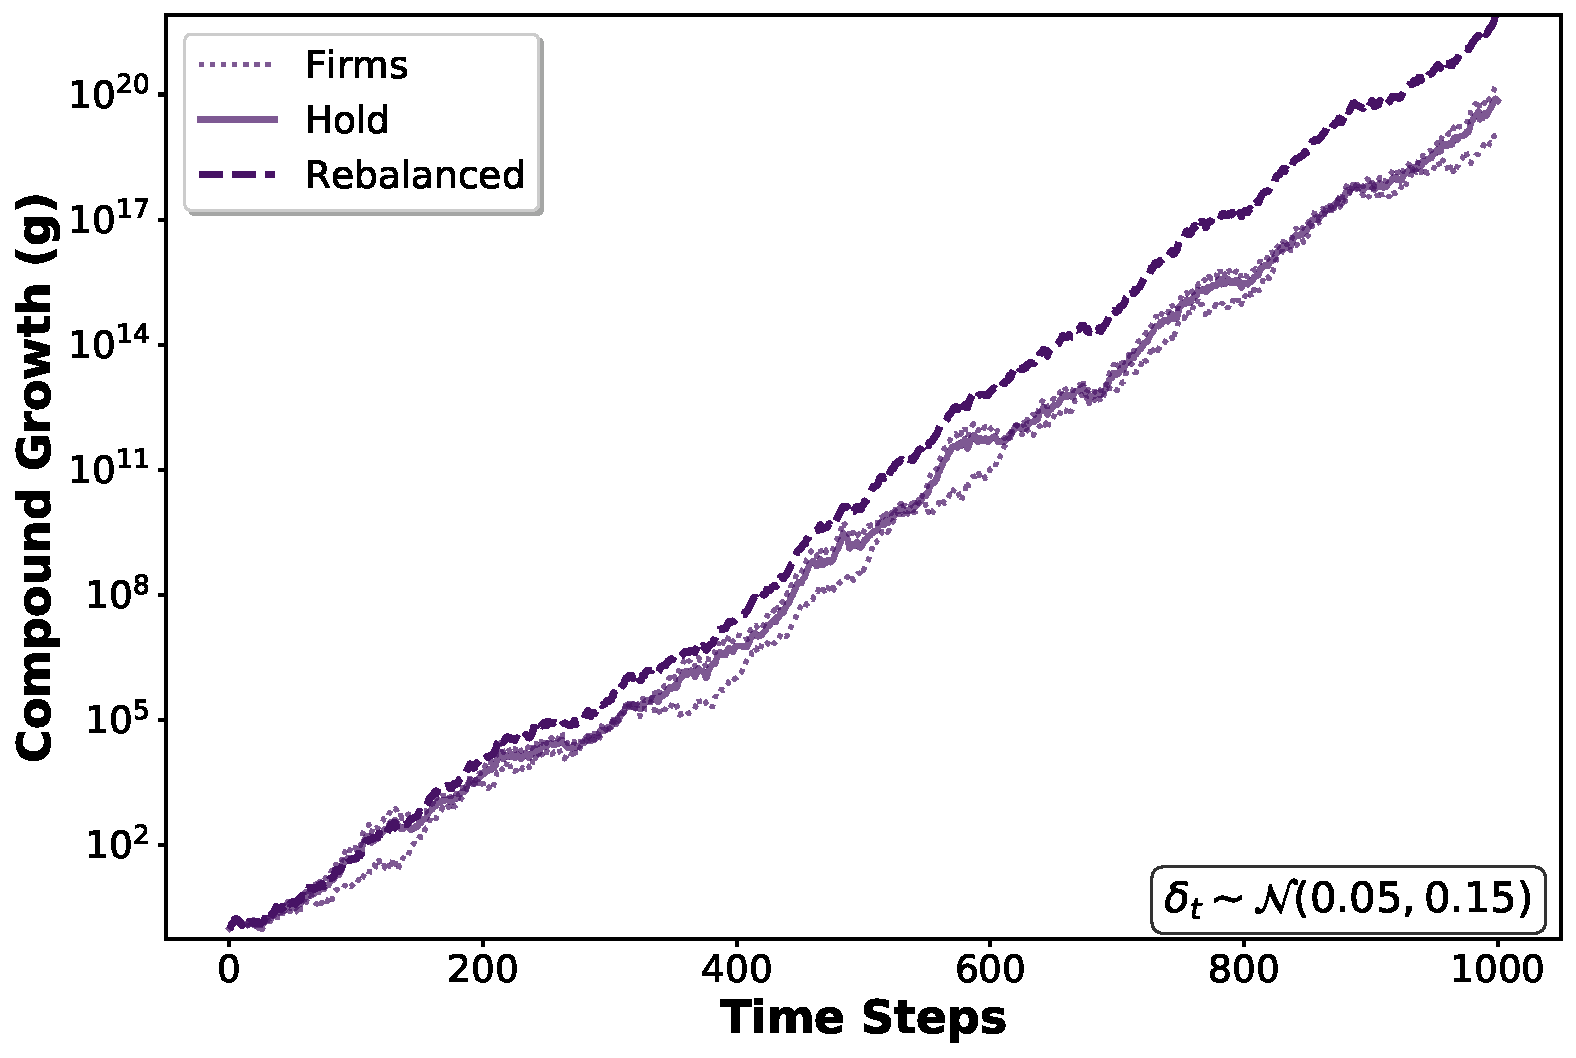
\includegraphics[width=0.75\textwidth]{figures/mc_figures/narrative_02_2assets_rebalanced}}
%     \only<3>{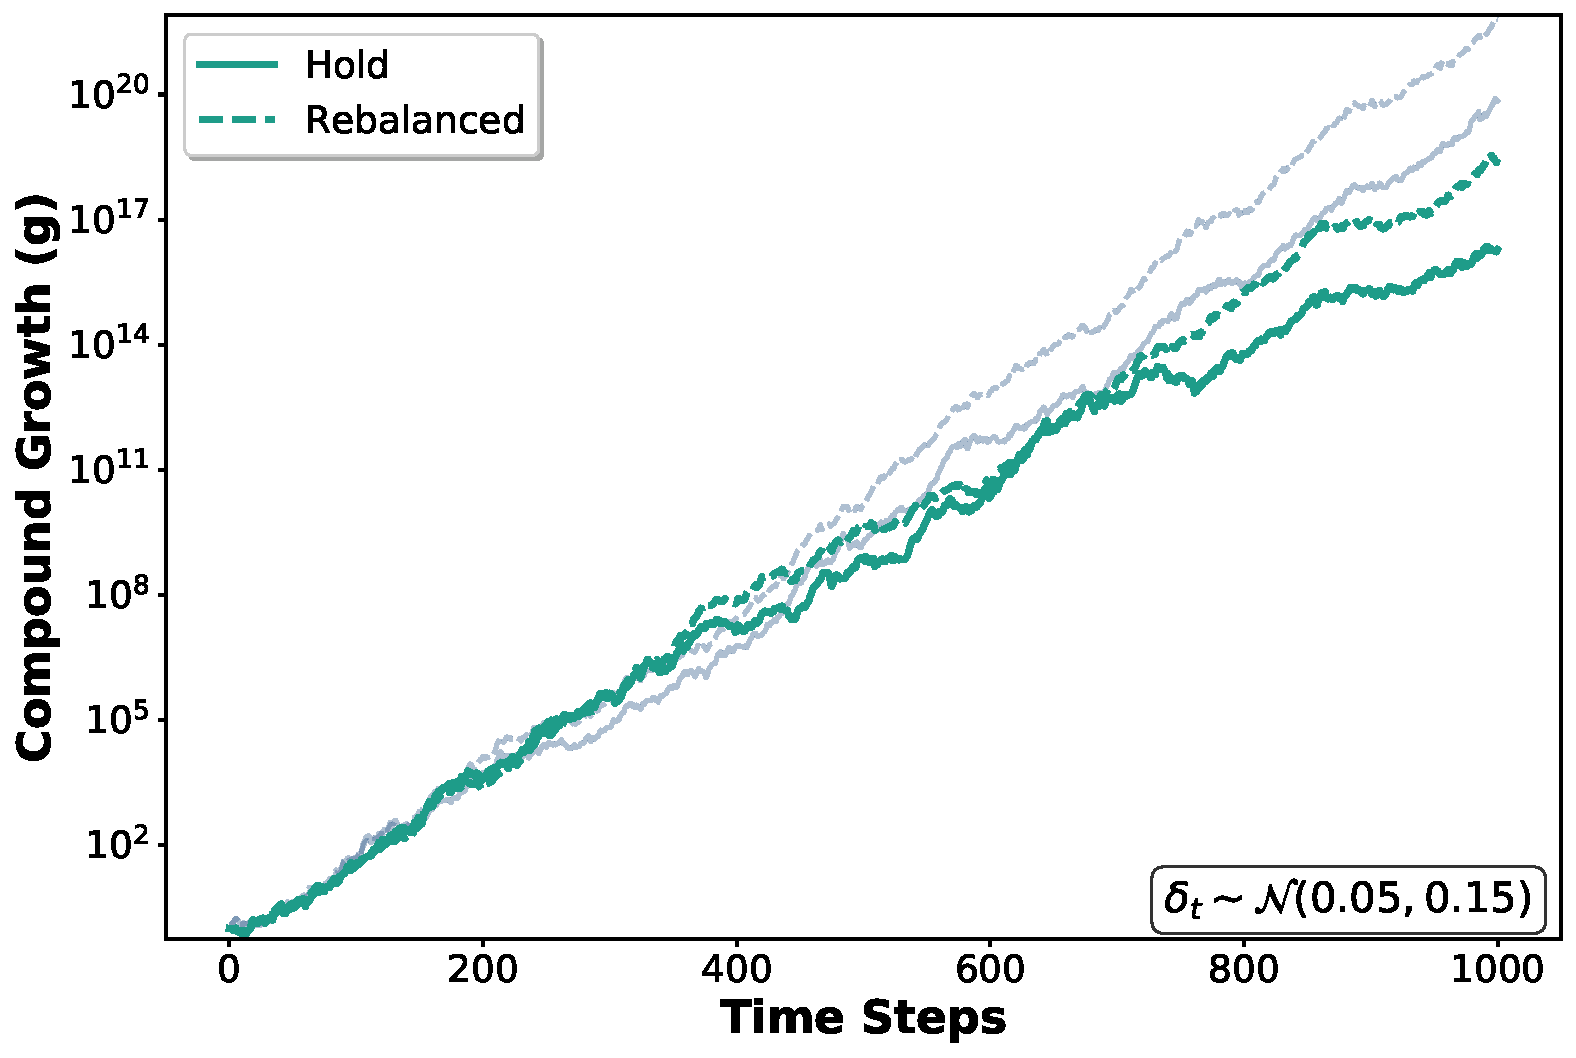
\includegraphics[width=0.75\textwidth]{figures/mc_figures/narrative_03_2assets_second}}
%     \only<4>{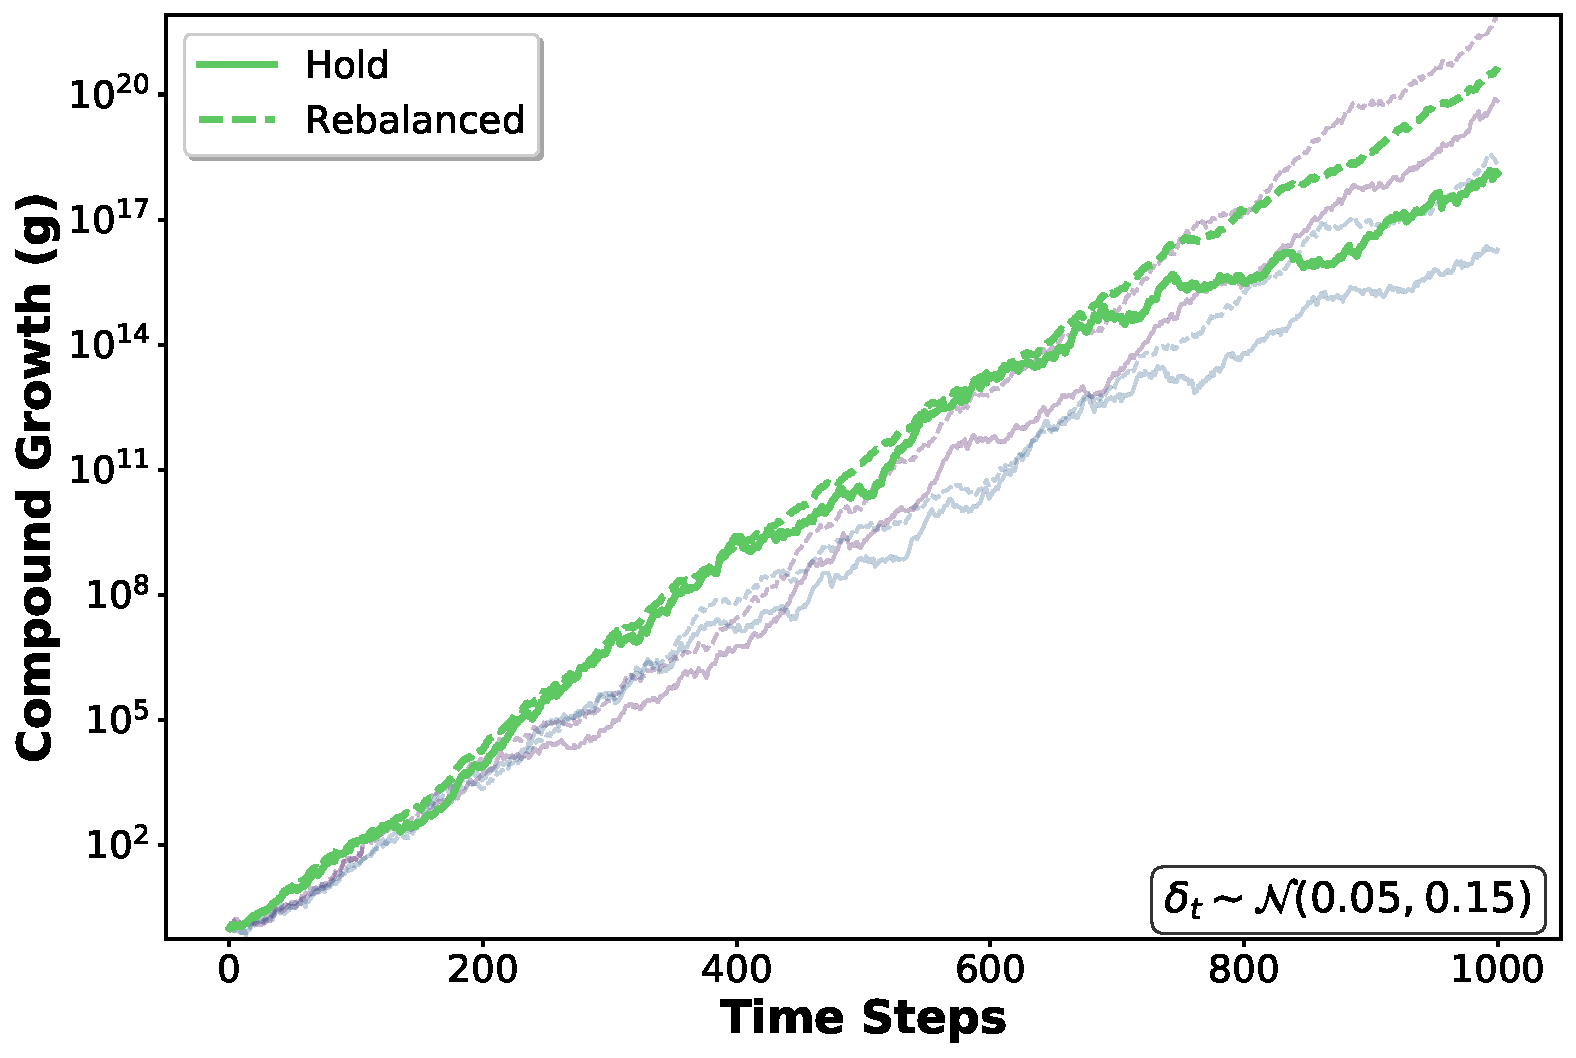
\includegraphics[width=0.75\textwidth]{figures/mc_figures/narrative_04_5assets}}
%     \only<5>{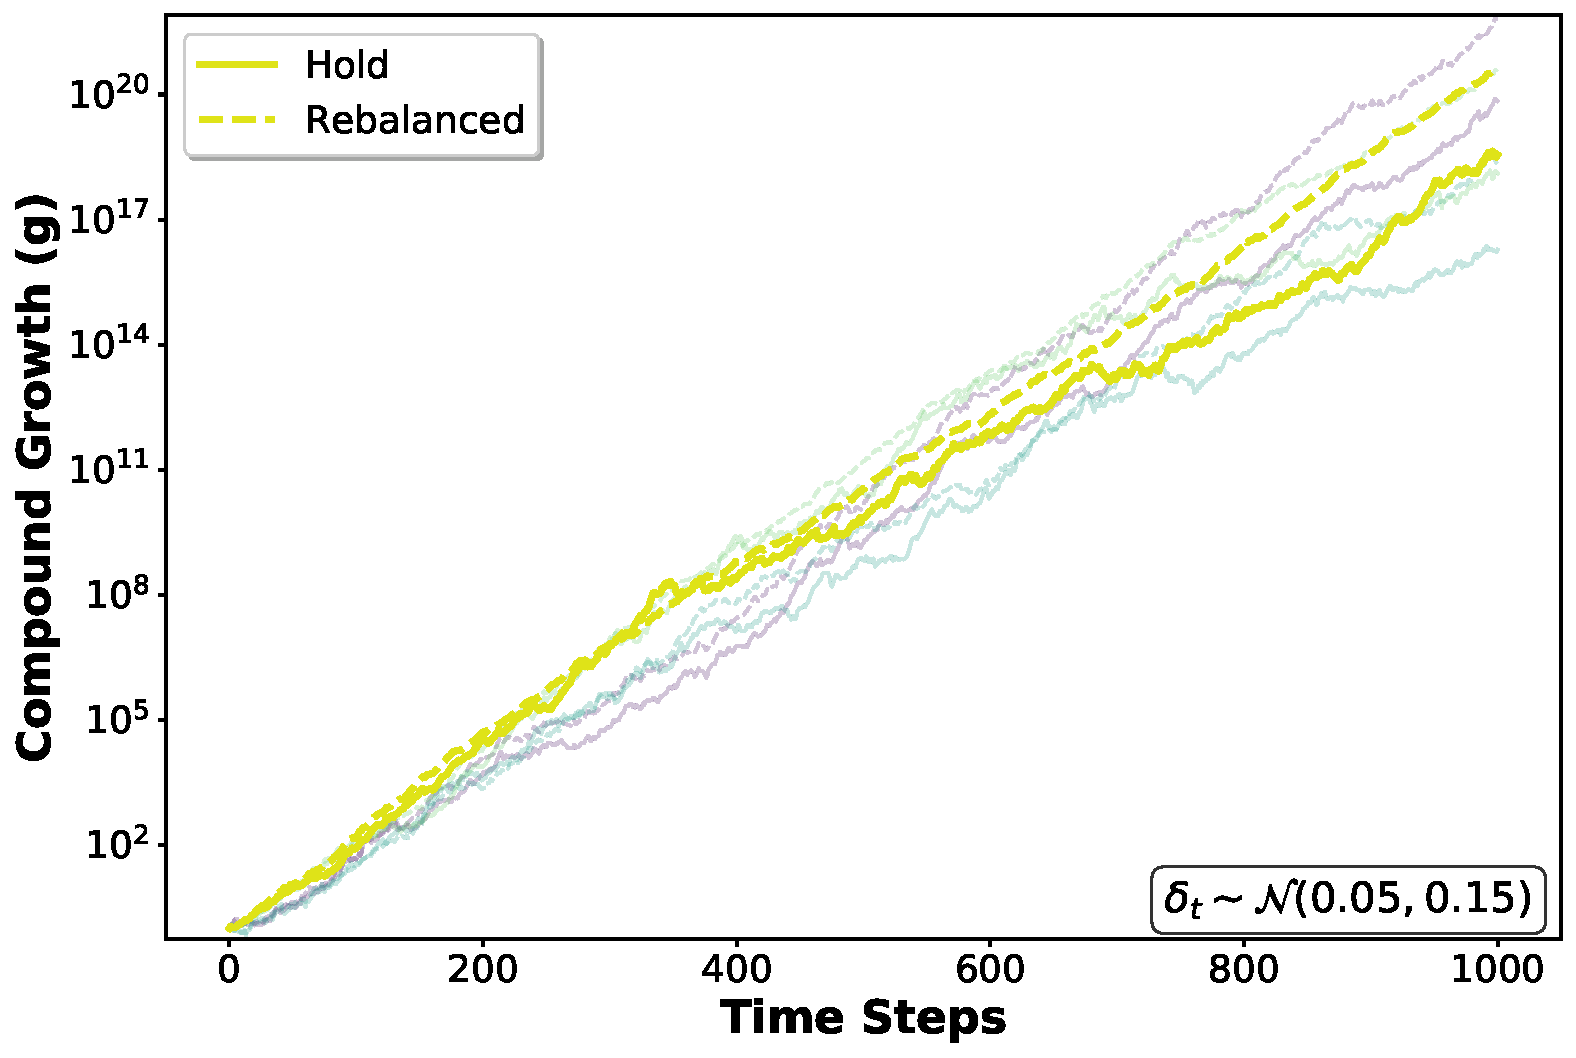
\includegraphics[width=0.75\textwidth]{figures/mc_figures/narrative_05_10assets}}
%   \end{center}
% \end{frame}


\begin{frame}{Multiplicative Growth}
  \begin{itemize}
    \onslide<1->{\item $g = \prod_{t=1}^T \delta_t$  instead of $g = \sum_{t=1}^T \delta_t$}
    \onslide<2->{\item ``When tomorrow depends on today'' $\rightarrow s_{t+1} = s_t \delta_t $ $\rightarrow$ The process of dependence} 
    \onslide<3->{\item All economic dynamics that are denoted in \% are usually linked to multiplicative dynamics}
    \onslide<4->{\item Prevalence of heavy tailed distributions in many economic domains well explained by multiplicativity}
    \onslide<5->{\item Examples of multiplicative processes
     \begin{itemize}
      \item Capital accumulation
      \item Trust, reputation
      \item Legal cases
     \end{itemize}} 
    \onslide<6->{\item Investment in capital goods don't just add capacity, it transforms the entire production structure}
  
  \end{itemize}
  
\end{frame}

\begin{frame}[fragile]{Growth and Risk: Two Sides of the Same Coin}
  \begin{columns}
   \begin{column}{0.6\textwidth}
    \begin{itemize}
      \setlength\itemsep{0.8em}
      
      \onslide<1->{\item Losses hurt exponentially more, while gains yield exponentially less ($\Delta_{g_1}} > \Delta_{g_2}$)} 
     \onslide<2->{\item Risk $\neq$ Volatility, Risk = Loss (large upswings aren't as important)} 
     \onslide<3->{\item Irreversibility of state transitions ($\delta_t = 0$) makes things even worse (think Russian Roulette)} 
     \onslide<4->{\item \alert{Shifting the return distribution upwards, avoiding very small growth increments}}
       
    \end{itemize}
   \end{column}
   \begin{column}{0.4\textwidth}
    \only<1->{\begin{tikzpicture}[scale=0.8]
        \begin{axis}[
            domain=1:10, % Domain of the function
            samples=100, % Number of samples for the function
            axis lines=middle, % Axis lines through the middle
            xlabel={$\delta$}, % Label for x-axis
            ylabel={$g$}, % Label for y-axis
            xtick=\empty, % Remove x-axis tick marks
            ytick=\empty, % Remove y-axis tick marks
            minor tick num=1, % Number of minor ticks
            enlargelimits={abs=0.5}, % Add some space around the plot
            every axis plot/.append style={thick}, % Thicker lines for plots
            clip=false,
        ]
            % Plot the logarithm function
            \addplot[blue, domain=0.3:10] {ln(x)};
    
            % Add points and vertical/horizontal lines
            \addplot[only marks, mark=*] coordinates {(2, 0.693) (4, 1.386) (7, 1.946) (9, 2.197)};
            \addplot[dashed] coordinates {(2,0) (2, 0.693)};
            \addplot[dashed] coordinates {(4,0) (4, 1.386)};
            \addplot[dashed] coordinates {(7,0) (7, 1.946)};
            \addplot[dashed] coordinates {(9,0) (9, 2.197)};

            \addplot[dashed] coordinates {(2, 0.693) (0, 0.693)};
            \addplot[dashed] coordinates {(4, 1.386) (0, 1.386)};
            \addplot[dashed] coordinates {(7, 1.946) (0, 1.946)};
            \addplot[dashed] coordinates {(9, 2.197) (0, 2.197)};

    
            % Add labels for the points
            \node at (axis cs:2, -0.02) [anchor=north] {$\delta_1 - x$};
            \node at (axis cs:4, -0.02) [anchor=north] {$\delta_1$};
            \node at (axis cs:7, -0.02) [anchor=north] {$\delta_2 - x$};
            \node at (axis cs:9, -0.02) [anchor=north] {$\delta_2$};

            \draw [decorate,decoration={brace,amplitude=10pt}] (axis cs:0, 0.693) -- (axis cs:0, 1.386) node [midway,left=10pt] {$\Delta_{g_1}$};
            \draw [decorate,decoration={brace,amplitude=10pt}] (axis cs:0, 1.946) -- (axis cs:0, 2.197) node [midway,left=10pt] {$\Delta_{g_2}$};    

    
        \end{axis}
        
    \end{tikzpicture}}
   \end{column}
  \end{columns}
 \end{frame}


 \begin{frame}{Sharing is Sparing}
  \begin{columns}
    \begin{column}{0.5\textwidth}
      \begin{itemize}
        \item Sharing (pooling) of resources reduces the impact of a loss $\rightarrow$ insurance
        \item \citet{peters2022ergodicity} show that with sharing under Gaussian growth increments we can increase $g = \mu - \frac{\sigma^2}{2}$ to $g = \mu - \frac{\sigma^2}{2N}$, with $N$ the number of sharing partners
        \item Giving up resources to reduce a loss can be worth more than the resources themselves (positive sum)
      \end{itemize}
      
    \end{column}
    \begin{column}{0.4\textwidth}
      \begin{tikzpicture}[firm/.style={draw, rectangle, minimum width=2.1cm, minimum
        height=0.6cm}
        ]


        \only<1>{\node[firm] (firmA) at (6, 8) {Firm A};
        \node[firm] (firmB) at (9, 8) {Firm B};

        \draw[dashed] (firmA) -- (firmB);

        \node (initA) at (6, 7.3) {100};
        \node (initB) at (9, 7.3) {100};

        \node (firstA) at (6, 5.3) {104};
        \node (firstB) at (9, 5.3) {99};
        
        \draw[->] (initA) -- (firstA) node[midway, left] {$\delta_{A1} = 4\%$};
        \draw[->] (initB) -- (firstB) node[midway, left] {$\delta_{B1} = -1\%$};

        \node[draw, ellipse, dotted] (pool) at (7.5,5.3) {203};

        \node (secondA) at (6, 3.3) {101.92};
        \node (secondB) at (9, 3.3) {101.97};

        \node[draw, ellipse, dotted] (pool1) at (7.5,2.3) {203.89};

        \draw[->] (firstA) -- (secondA) node[midway, left] {$\delta_{A2} = -2\%$};
        \draw[->] (firstB) -- (secondB) node[midway, left] {$\delta_{B2} = 3\%$};

        
        }


        \only<2>{\node[firm] (firmA) at (6, 8) {Firm A};
        \node[firm] (firmB) at (9, 8) {Firm B};

        \draw[dashed] (firmA) -- (firmB);

        \node (initA) at (6, 7.3) {100};
        \node (initB) at (9, 7.3) {100};

        
        \node (firstA) at (6, 6.3) {104};
        \node (firstB) at (9, 6.3) {99};
        
        \draw[->] (initA) -- (firstA) node[midway, left] {$\delta_{A1} = 4\%$};
        \draw[->] (initB) -- (firstB) node[midway, left] {$\delta_{B1} = -1\%$};

        \node[draw, ellipse] (pool) at (7.5,5.3) {203};

        \draw[->, shorten >=4pt] (firstA) -- (pool.north);
        \draw[->, shorten >=4pt] (firstB) -- (pool.north);

        \node (afterA) at (6, 4.3) {101.5};
        \node (afterB) at (9, 4.3) {101.5};

        \draw[->] (pool.south) -- (afterA);
        \draw[->] (pool.south) -- (afterB);

        \node (secondA) at (6, 3.3) {99.47};
        \node (secondB) at (9, 3.3) {104.545};

        \draw[->] (afterA) -- (secondA) node[midway, left] {$\delta_{A2} = -2\%$};
        \draw[->] (afterB) -- (secondB) node[midway, left] {$\delta_{B2} = 3\%$};

        \node[draw, ellipse] (pool1) at (7.5,2.3) {204.015};

        \draw[->, shorten >=4pt] (secondA) -- (pool1.north);
        \draw[->, shorten >=4pt] (secondB) -- (pool1.north);}





        
      \end{tikzpicture}
      
    \end{column}
  \end{columns}
  
 \end{frame}

 \begin{frame}{The Anatomy of an Agent Based Model}
  \begin{tikzpicture}[
    market/.style={draw, rectangle, minimum width=2.2cm, minimum
  height=0.7cm},
    firm/.style={draw, rectangle, minimum width=2.2cm, minimum
  height=0.7cm}
  ]
    \node[market] (market1) at (0,3) {Market 1};
    \node[market] (market2) at (0,2) {Market 2};
    \node[market] (market3) at (0,1) {Market 3};
    \node at (0,0) {$\vdots$};
    \node[market] (marketM1) at (0,-1) {Market M-1};
    \node[market] (marketM) at (0,-2) {Market M};

    \node at (0, -2.8)  {$\mathcal{N}(\mu_m, \sigma_m)$};


    \only<1>{\node[firm] (firm1_1) at (3.5,3) {Firm 1};
    \node[firm] (firm2) at (3.5,2) {Firm 2};
    \node[firm] (firm3) at (3.5,1) {Firm 3};
    \node at (3.5,0) {$\vdots$};
    \node[firm] (firmN1) at (3.5,-1) {Firm N-1};
    \node[firm] (firmN_1) at (3.5,-2) {Firm N};

    \node at (3.5, -2.8)  {$\mathcal{N}(\mu_1, \sigma_1)$};

    \draw[
    decorate,
    decoration={
      brace,
      raise=8pt,
      amplitude=7pt,
      aspect=0.065,
      mirror
    }
    ] (firm1_1.north west) -- (firmN_1.south west);}

    \only<2>{
    \node[firm] (firm1_2) at (3.5,3) {Firm 1};
    \node[firm] (firm2) at (3.5,2) {Firm 2};
    \node[firm] (firm3) at (3.5,1) {Firm 3};
    \node at (3.5,0) {$\vdots$};
    \node[firm] (firmN1) at (3.5,-1) {Firm N-1};
    \node[firm] (firmN_2) at (3.5,-2) {Firm N};

    \node at (3.5, -2.8)  {$\mathcal{N}(\mu_3, \sigma_3)$};

    \draw[
    decorate,
    decoration={
      brace,
      raise=8pt,
      amplitude=7pt,
      aspect=0.41,
      mirror
    }
    ] (firm1_2.north west) -- (firmN_2.south west);}

    \only<3>{
      
      \node[firm] (firm5) at (3.5,3) {Firm 5};
      \node[firm] (firm27) at (3.5,2) {Firm 27};
      \node[firm] (firm70) at (3.5,-2) {Firm 70};
      
      \node[draw, fit=(firm5)(firm27)(firm70), rectangle, dashed, inner
        sep=10pt] (conglomerate) {};

      \node at (3.5, 0) {Conglomerate};

      \draw[->] (market1) -- (firm5);
      \draw[->] (market2) -- (firm27);
      \draw[->] (marketM) -- (firm70);



    }
      

    
    
  \end{tikzpicture}
 \end{frame}



\begin{frame}{Growing in the Markets}
  \begin{tikzpicture}[firm/.style={draw, rectangle, minimum width=2.1cm, minimum
        height=0.6cm}
        ]
    \only<1->{
      
    \node[firm] (firm) at (0,2) {Firm$_{im}$};

    \node at (2.5, 2) {$\delta_{it} \sim \mathcal{N}(\mu_m, \sigma_m)$};
  
        
    \node (revenue) at (0, 0.5) {$\Delta_{it} = s_{it-1} \delta_{it} - s_{it-1}$};
    }

    \node[opacity=0] (blank1) at (0, -2.5) {1};
    \node[opacity=0] (blank2) at (3.5,-1) {1};

    \node[draw, fit=(firm)(revenue)(blank1)(blank2), rectangle, dashed, inner sep=10pt] {};
    
    
    \only<2->{\node (profit1) at (-1, -1) {$\Pi_{it} = \Delta_{it}$};

    \draw[->] (revenue) -- (profit1);
    }
    
    
    

    


    \only<3->{

    \node[firm] (cong) at (8,2) {Conglomerate$_{c}$};

    \node (sumShared) at (6, 0.5) {$\sum_{i \in c} \alpha \Delta_{it}$};
    
    \draw[->] (revenue) -- (sumShared);
    
    
    \node (costCong) at (10, 0.5) {$\Phi(O_c, M) = \frac{1}{1 + e^{|O_c| + 0.4 M}}$};

    \node (pool) at (8, -1) {$\Omega_{ct} = \sum_{i \in c} \alpha \Delta_{it} -  \Phi(O_c, M) \sum_{i \in c} s_{it}$};

    \draw[->] (sumShared) -- (pool);
    \draw[->] (costCong) -- (pool);

    \node[opacity=0] (blank3) at (8, 2) {1};
    \node[opacity=0] (blank4) at (8,-2.5) {1};

    \node[draw, fit=(sumShared)(costCong)(pool)(blank3)(blank4), rectangle, dashed, inner sep=10pt] {};

    }

    \only<4->{

    \node (profit2) at (2,-1) {$\Pi_{it} = (1 - \alpha) \Delta_{it} +
  \frac{\Omega_{ct}}{|O_{c_i}|}$};

    \draw[->] (pool) -- (profit2);
    }

    \only<5->{
    \node (nextState) at (0, -2.5) {$s_{it} = s_{it-1} + \Pi_{it}$};
    \draw[->] (profit1) -- (nextState);
    \draw[->] (profit2) -- (nextState);
    }


  \end{tikzpicture}
  
\end{frame}
 


\begin{frame}{Merging and Splitting}
  \begin{tikzpicture}
    [firm/.style={draw, rectangle, minimum width=2.1cm, minimum
        height=0.6cm, node distance=0.5cm}
        ]

    \only<1->{

    \node[firm] (firm) at (0,0.4) {Firm$_{im}$};
    \node at (0,-0.5) {$p=5\%$};
 
    \node[opacity=0] (blank1) at (2.5,0.4) {};

    \draw[->] (firm.est) -- (blank1);


    \node[draw, rectangle, dotted] (feasibilityCheck) at (3.5, 3) {Feasibility};

    \node[below=of feasibilityCheck] (select) {Pick $j \in (M \times N ) - 1$};

    \node[below=of select] (nonSame){$m_i \neq m_j$};
    
    \node[below=of nonSame] (nonCong){$(O_{c_i} \cap O_{c_j} = \emptyset)$};

    \draw[->] (select) -- (nonSame);
    \draw[->] (nonSame) -- (nonCong);


    \node[draw, fit=(feasibilityCheck)(feasibilityCheck)(nonSame)(nonCong), rectangle, dashed, inner sep=10pt, text width=3cm] {};

    }

    \only<2->{

    \node[draw, rectangle, dotted, right=1.87cm of feasibilityCheck] (desirabilityCheck) {Desirability};

    \node[below=of desirabilityCheck] (synthPool) {Compute $\hat{\Omega}$};
    
    \node[below=of synthPool] (checkPools) {$\hat{\Omega} > \Omega$};

    \node[below=of checkPools] (merge) {\textbf{Merge}};

    \draw[->] (synthPool) -- (checkPools);
    \draw[->] (checkPools) -- (merge);

    \node[draw, fit=(desirabilityCheck)(synthPool)(checkPools)(merge), rectangle, dashed, inner sep=10pt, text width=3cm] {};

    \node[opacity=0] (blank2) at (4.5,0.4) {};
    \node[opacity=0] (blank3) at (6.5,0.4) {};
    
    \draw[->] (blank2) -- (blank3);

    }

    \only<3->{

    \node[draw, rectangle, dotted, right=2cm of desirabilityCheck] (split) {Splitting};

    \node[below=of split] (compRate) {Compute $\hat{g}_{i(t-l):t}$};

    \node[below=of compRate] (checkRates)  {$\hat{g}_{i(t-l):t} > g_{i(t-l):t}$};

    \node[below=of checkRates] (exit)  {\textbf{Exit}};

    \draw[->] (compRate) -- (checkRates);
    \draw[->] (checkRates) -- (exit);


    \node[draw, fit=(split)(exit)(compRate)(checkRates), rectangle, dashed, inner sep=10pt, text width=3cm] {};

    }
    
  \end{tikzpicture}
\end{frame}

\begin{frame}{Parametrization and Experimental Setup}
  \begin{columns}
    \begin{column}{0.5 \textwidth}
      \begin{table}[h]
        \centering
        \begin{tabular}{|c|c|}
          \hline
          \textbf{Parameter} & \textbf{Value} \\
          \hline
          $M$ & 100  \\
          $N$ & 100 \\
          $T$ & 1000 \\
          $l$ & 50 \\
          $p$ & 0.05 \\
          $\alpha$ & $\left[0, 0.5 \right]$ \\
          \hline
        \end{tabular}
      \end{table}
    \end{column}
    \begin{column}{0.5 \textwidth}
      \begin{itemize}
        \item 100 Markets means maximum conglomerate size is 100
        \item Increase the sharing rate $\alpha$ by $0.02$
        \item Run each parametrization 10 times and average along their trajectories
        \item Management cost function set such that operating in 40\,\% of the markets cost 50\,\% of the conglomerate each step
      \end{itemize}
      
    \end{column}
  \end{columns}

  
  
\end{frame}


\begin{frame}{Merging Behavior}
  \begin{columns}
    \begin{column}{0.6\textwidth}
      \centering
      \begin{figure}
        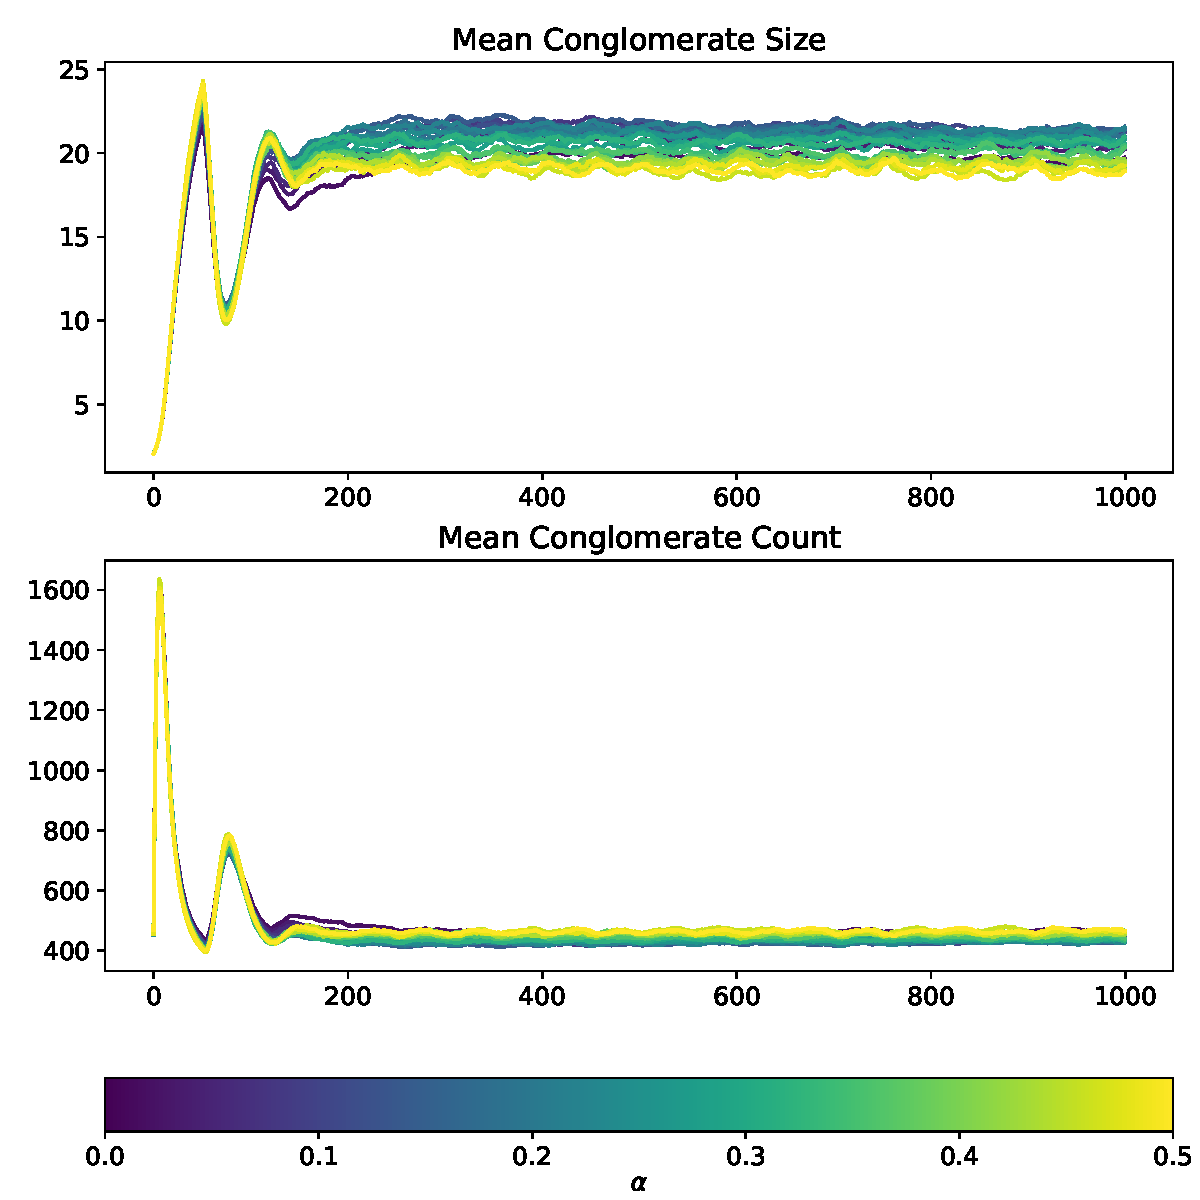
\includegraphics[width=8.5cm]{figures/sizes.pdf}
      \end{figure}
    \end{column}
    \begin{column}{0.45\textwidth}
      \begin{itemize}
        \item Stable conglomerate size
        \item Stable number of conglomerates
        \item Stabilization after the initial $l$ review periods
        \item Increasing $\alpha$ decreases conglomerate size
        \item Increasing $\alpha$ marginally decreases conglomerate count
      \end{itemize}
      
    \end{column}
  \end{columns}

\end{frame}

\begin{frame}{The Impact of the Pooling Rate on Market Shares}
  \begin{columns}
    \begin{column}{0.6\textwidth}
      \centering
      \begin{figure}
        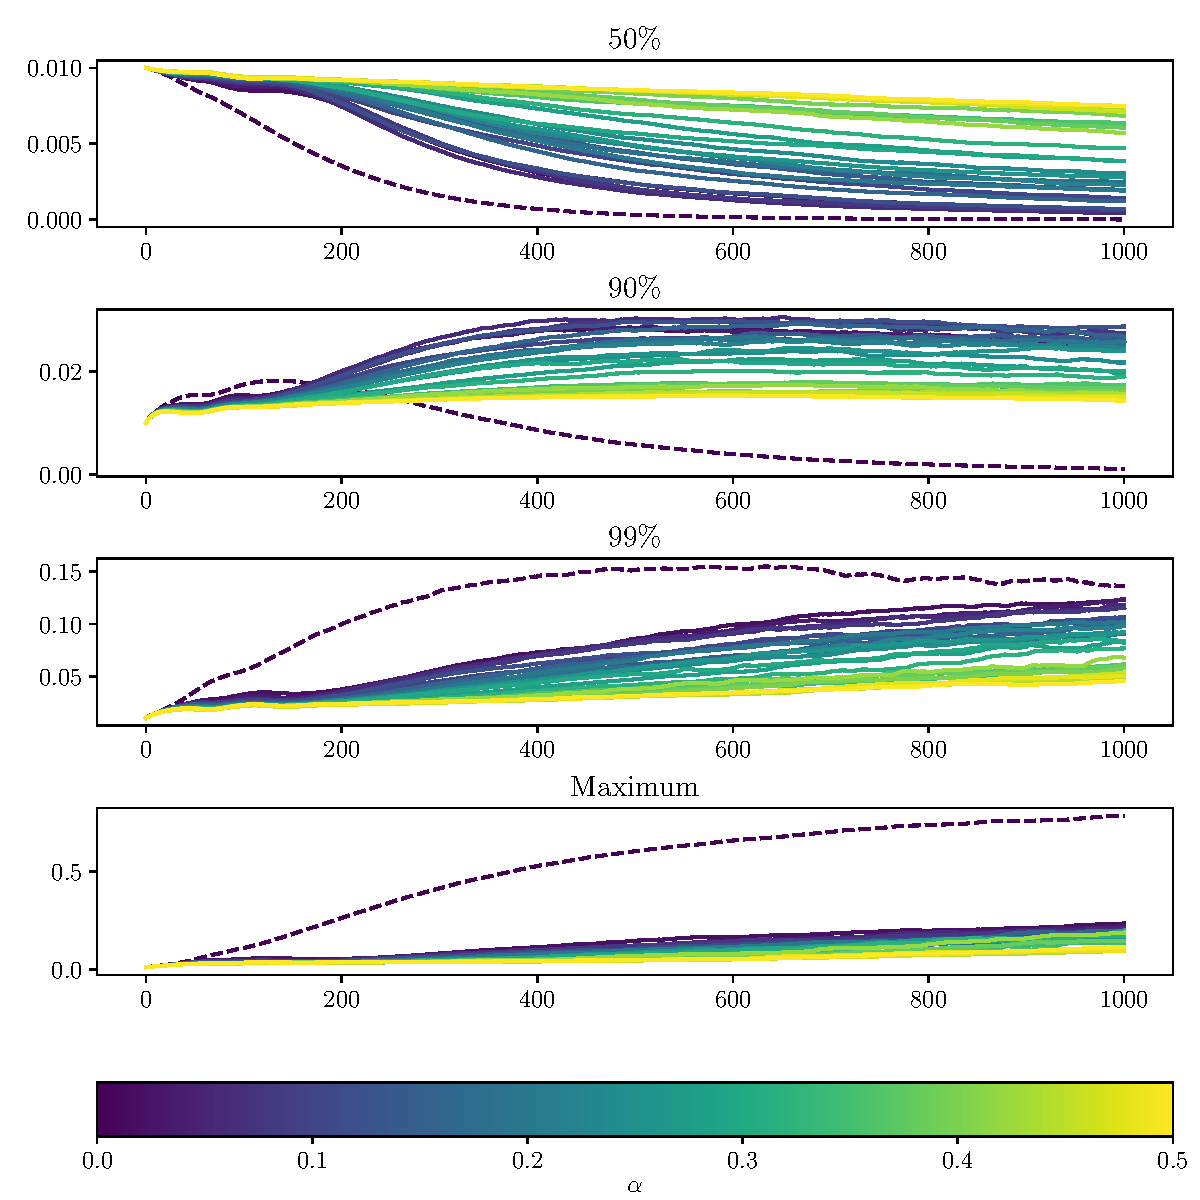
\includegraphics[width=8.5cm]{figures/shares.pdf}
      \end{figure}
    \end{column}
    \begin{column}{0.45\textwidth}
      \begin{itemize}
        \item Perfect equality is $0.01$ with 100 firms per market
        \item Inequality increases with time
        \item Non-pooling returns the expected log-normal distribution
        \item Increasing $\alpha$ decreases market share inequality and slows increase over time
      \end{itemize}
      
    \end{column}
  \end{columns}
\end{frame}

\begin{frame}{Conglomerate Size and Market Share}
  \begin{columns}
    \begin{column}{0.6\textwidth}
      \centering
      \begin{figure}
        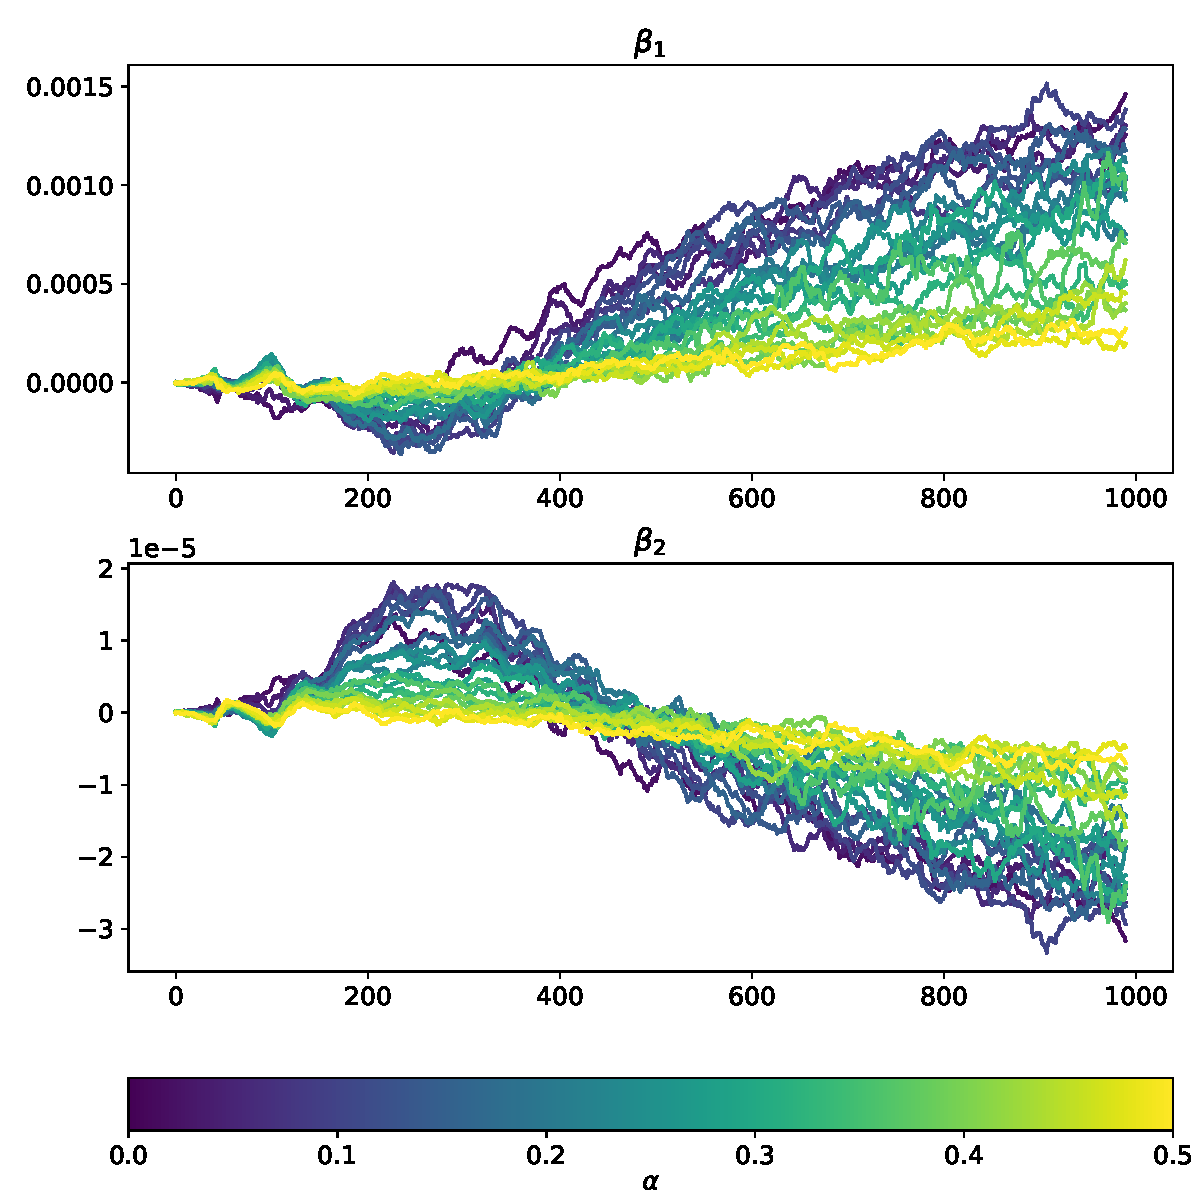
\includegraphics[width=8.5cm]{figures/ests.pdf}
      \end{figure}
    \end{column}
    \begin{column}{0.45\textwidth}
      \begin{itemize}
        \item Impact of conglomerate size on market share of firms within the conglomerate $\bar{\Omega}_{ct} = \beta_{0t} + \beta_{1t} |O_{ct}| + \beta_{2t} |O_{ct}|^2$
        \item $\beta_1 > 0$: Variance reduction
        \item $\beta_2 < 0$: Management cost
        \item Increasing $\alpha$ decreases the effects as market shares tend to equalize $\rightarrow$ lower market concentration
      \end{itemize}

      
    \end{column}
  \end{columns}

\end{frame}



\begin{frame}{The Impact of the Pooling Rate on Mobility}
  \begin{columns}
    \begin{column}{0.6\textwidth}
      \centering
      \begin{figure}
        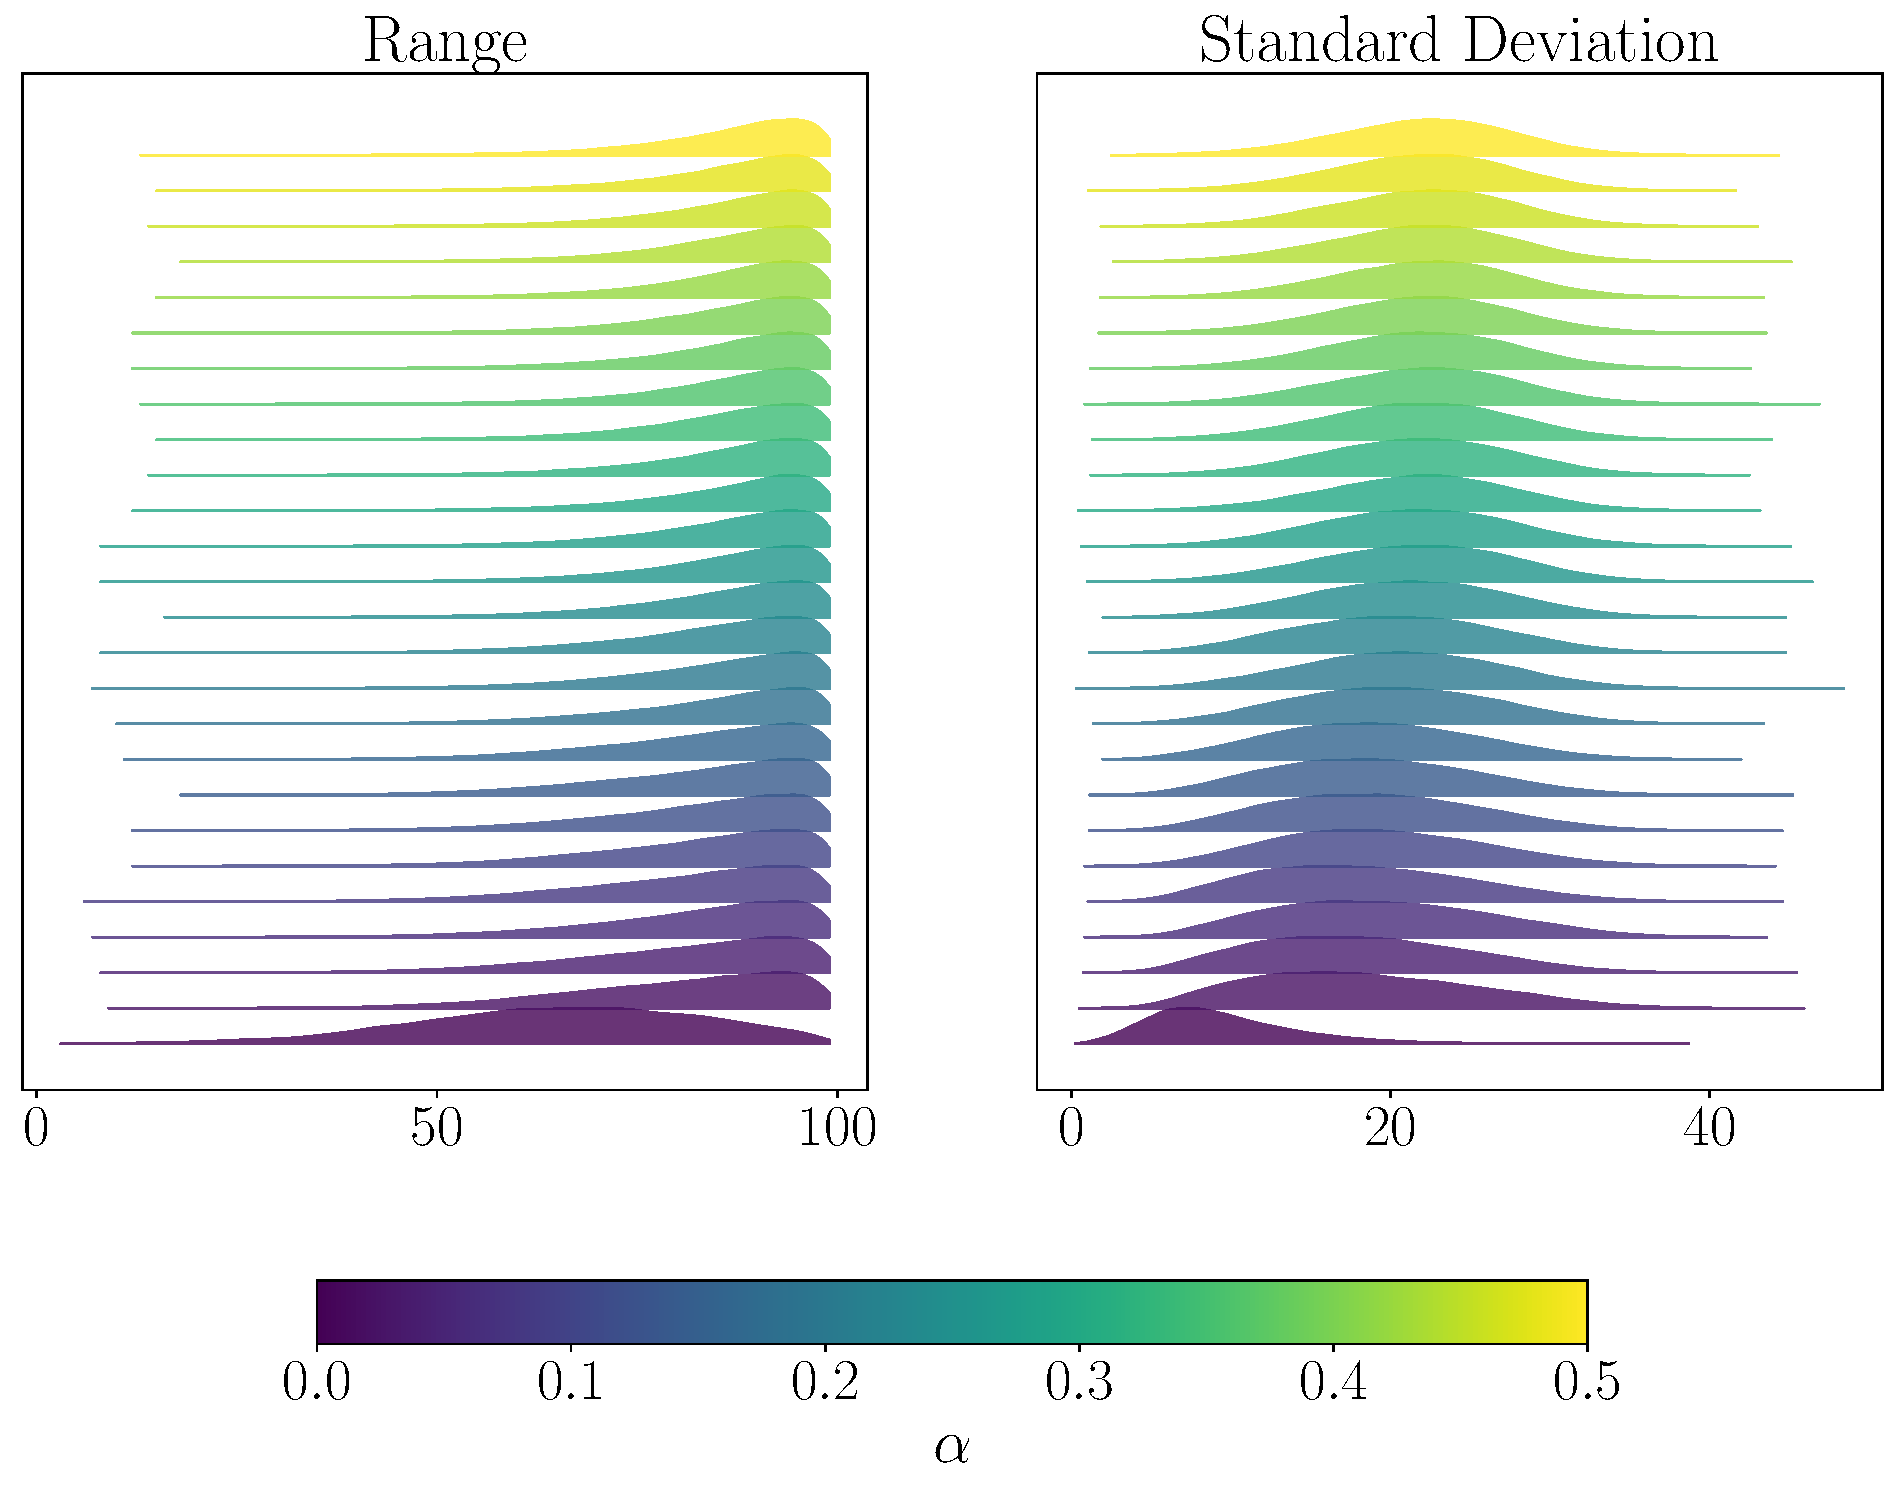
\includegraphics[width=8.5cm]{figures/mobility.pdf}
      \end{figure}
    \end{column}
    \begin{column}{0.45\textwidth}
      \begin{itemize}
        \item Range as the difference between ranks over time
        \item Standard deviation of ranks over time 
        \item Any $\alpha > 0$ improves mobility drastically
        \item Increasing $\alpha$ shifts distribution to higher mobility
        \item Increasing $\alpha$ decreases the spread of distribution 
        \item Decreases barriers to entry
      
      \end{itemize}
    \end{column}
  \end{columns}

\end{frame}


\begin{frame}{Key Findings}
  
  \begin{enumerate}
    \setlength\itemsep{0.8em}
    \item Growth rate optimization is a novel view in standard models of industrial organization
    \item Growth rate optimization through resource sharing is a possible reason why conglomerates form
    \item Pooling of resources within the conglomerate allows for improved performance for all companies with it 
    \item Increasing firm cooperation through conglomerate formation improves static and dynamic measures of competitiveness
    \item Management costs play a crucial role in determining the size of a conglomerate
  \end{enumerate}

\end{frame}


\begin{frame}{Future Developments}
    \begin{enumerate}
        \setlength\itemsep{0.8em}
        \item Other resources outside of capital could be modelled
        \item Include jump processes or other return distributions
        \item Robust management cost function for conglomerate size
        \item More guided merger targeting process
        \item Investigate how conglomerates change barriers to entry
    \end{enumerate}
\end{frame}

  \begin{frame}[allowframebreaks]{References}
      \bibliographystyle{apalike}  % or plainnat, abbrvnat, etc.
      \bibliography{references}    % points to your references.bib file
  \end{frame}


\begin{frame}
  \begin{columns}
    \begin{column}{0.5\textwidth}
    \textbf{\Huge Reach Out!}

    \medskip

    \vspace{1.5cm}

    \href{mailto:simon.bloethner@uni-bayreuth.de}{simon.bloethner@uni-bayreuth.de}
    
    \end{column}
      \begin{column}{0.5\textwidth}
        \begin{figure}
          
\includegraphics[width=0.8\textwidth]{figures/LI_QR.JPG}
        \end{figure}
  \end{column}
    
  \end{columns}
\end{frame}

\end{document}